\documentclass[a4paper,12pt,headsepline]{scrartcl}
\usepackage{tikz}
\usepackage{tikz-qtree}
\usepackage{fix-cm}
\begin{document}
\begin{center} 
\begin{tabular}{l}$A\rightarrow S C~~$\\ 
$B\rightarrow S S~~$\\ 
$S\rightarrow b~|~S B~|~a~~$\\ 
$C\rightarrow S S~~$\\ 
\end{tabular} 
\end{center}
\begin{center}
\resizebox{\linewidth}{!}{
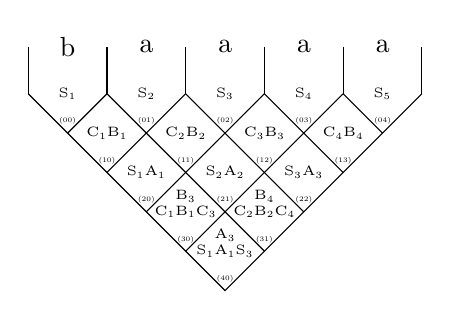
\begin{tikzpicture}[baseline]
\newcommand{\myfontvars}[1]{
\fontsize{4.9}{12}\selectfont{#1}
}\newcommand{\myfontnumbering}[1]{
\fontsize{2.5}{12}\selectfont{#1}
}%Outer hull
%Tip of the pyramid
\coordinate (tip) at (2.5,-2.5);
\foreach \i in {0,...,5} {
 	\coordinate (\i) at (\i,0);
}
%Draw the left and right line of the pyramid pointing downwards
\draw (0) -- (tip) -- (5);
%Grid lines direction down-left to top-right
\coordinate (dl1) at (0.5,-0.5);
\coordinate (dl2) at (1.0,-1.0);
\coordinate (dl3) at (1.5,-1.5);
\coordinate (dl4) at (2.0,-2.0);
\draw (dl1) -- (1,0);
\draw (dl2) -- (2,0);
\draw (dl3) -- (3,0);
\draw (dl4) -- (4,0);
%Grid lines direction down-right to top-left
\coordinate (dr1) at (3.0,-2.0);
\coordinate (dr2) at (3.5,-1.5);
\coordinate (dr3) at (4.0,-1.0);
\coordinate (dr4) at (4.5,-0.5);
\draw (dr1) -- (1,0);
\draw (dr2) -- (2,0);
\draw (dr3) -- (3,0);
\draw (dr4) -- (4,0);
%Small lines at the top
\coordinate (top0) at (0.0,0.0);
\coordinate (top1) at (1.0,0.0);
\coordinate (top2) at (2.0,0.0);
\coordinate (top3) at (3.0,0.0);
\coordinate (top4) at (4.0,0.0);
\coordinate (top5) at (5.0,0.0);
\coordinate (topUpper0) at (0.0,0.6);
\coordinate (topUpper1) at (1.0,0.6);
\coordinate (topUpper2) at (2.0,0.6);
\coordinate (topUpper3) at (3.0,0.6);
\coordinate (topUpper4) at (4.0,0.6);
\coordinate (topUpper5) at (5.0,0.6);
\draw (top0) -- (topUpper0);
\draw (top1) -- (topUpper1);
\draw (top2) -- (topUpper2);
\draw (top3) -- (topUpper3);
\draw (top4) -- (topUpper4);
\draw (top5) -- (topUpper5);
%The string
\coordinate (w0) at (0.5,0.6);
\coordinate (w1) at (1.5,0.6);
\coordinate (w2) at (2.5,0.6);
\coordinate (w3) at (3.5,0.6);
\coordinate (w4) at (4.5,0.6);
\node [] at (w0) {b};
\node [] at (w1) {a};
\node [] at (w2) {a};
\node [] at (w3) {a};
\node [] at (w4) {a};
% Variables in the cells
%cells00
\coordinate (center00) at (0.5,0.0);
\node [below=0.18cm] at (center00) {\myfontnumbering{$(00)$}};
\node [] at (center00) {\myfontvars{S$_{1}$}};
%cells01
\coordinate (center01) at (1.5,0.0);
\node [below=0.18cm] at (center01) {\myfontnumbering{$(01)$}};
\node [] at (center01) {\myfontvars{S$_{2}$}};
%cells02
\coordinate (center02) at (2.5,0.0);
\node [below=0.18cm] at (center02) {\myfontnumbering{$(02)$}};
\node [] at (center02) {\myfontvars{S$_{3}$}};
%cells03
\coordinate (center03) at (3.5,0.0);
\node [below=0.18cm] at (center03) {\myfontnumbering{$(03)$}};
\node [] at (center03) {\myfontvars{S$_{4}$}};
%cells04
\coordinate (center04) at (4.5,0.0);
\node [below=0.18cm] at (center04) {\myfontnumbering{$(04)$}};
\node [] at (center04) {\myfontvars{S$_{5}$}};
%cells10
\coordinate (center10) at (1.0,-0.5);
\node [below=0.18cm] at (center10) {\myfontnumbering{$(10)$}};
\node [] at (center10) {\myfontvars{C$_{1}$B$_{1}$}};
%cells11
\coordinate (center11) at (2.0,-0.5);
\node [below=0.18cm] at (center11) {\myfontnumbering{$(11)$}};
\node [] at (center11) {\myfontvars{C$_{2}$B$_{2}$}};
%cells12
\coordinate (center12) at (3.0,-0.5);
\node [below=0.18cm] at (center12) {\myfontnumbering{$(12)$}};
\node [] at (center12) {\myfontvars{C$_{3}$B$_{3}$}};
%cells13
\coordinate (center13) at (4.0,-0.5);
\node [below=0.18cm] at (center13) {\myfontnumbering{$(13)$}};
\node [] at (center13) {\myfontvars{C$_{4}$B$_{4}$}};
%cells20
\coordinate (center20) at (1.5,-1.0);
\node [below=0.18cm] at (center20) {\myfontnumbering{$(20)$}};
\node [] at (center20) {\myfontvars{S$_{1}$A$_{1}$}};
%cells21
\coordinate (center21) at (2.5,-1.0);
\node [below=0.18cm] at (center21) {\myfontnumbering{$(21)$}};
\node [] at (center21) {\myfontvars{S$_{2}$A$_{2}$}};
%cells22
\coordinate (center22) at (3.5,-1.0);
\node [below=0.18cm] at (center22) {\myfontnumbering{$(22)$}};
\node [] at (center22) {\myfontvars{S$_{3}$A$_{3}$}};
%cells30
\coordinate (center30) at (2.0,-1.5);
\node [below=0.18cm] at (center30) {\myfontnumbering{$(30)$}};
\node [] at (center30) {\myfontvars{C$_{1}$B$_{1}$C$_{3}$}};
\node [above] at (center30) {\myfontvars{B$_{3}$}};
%cells31
\coordinate (center31) at (3.0,-1.5);
\node [below=0.18cm] at (center31) {\myfontnumbering{$(31)$}};
\node [] at (center31) {\myfontvars{C$_{2}$B$_{2}$C$_{4}$}};
\node [above] at (center31) {\myfontvars{B$_{4}$}};
%cells40
\coordinate (center40) at (2.5,-2.0);
\node [below=0.18cm] at (center40) {\myfontnumbering{$(40)$}};
\node [] at (center40) {\myfontvars{S$_{1}$A$_{1}$S$_{3}$}};
\node [above] at (center40) {\myfontvars{A$_{3}$}};
\end{tikzpicture}
}
\end{center}
\begin{center}
\resizebox{\linewidth}{!}{
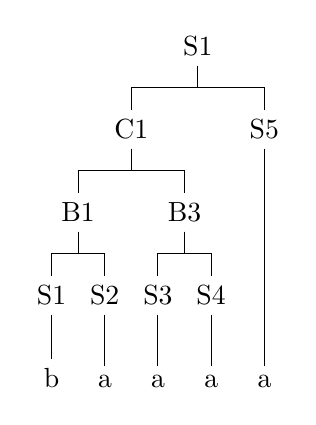
\begin{tikzpicture}[baseline]
		\tikzset{frontier/.style={distance from root=120pt}} %height of tree times 30pt
		\tikzset{edge from parent/.style= {
				draw,
				edge from parent path={(\tikzparentnode.south)	-- +(0,-8pt)-| (\tikzchildnode)}
			}
		}
		\Tree
[.S1
[.C1
[.B1
[.S1 b ]
[.S2 a ]
]
[.B3
[.S3 a ]
[.S4 a ]
]
]
[.S5 a ]
]
\end{tikzpicture}
}
\end{center}
\end{document}
